\pagebreak
\subsection{Thermal Design} \label{Thermal_section}
\subsubsection{Optothermal considerations}

In order to ensure minimise measurement error in acquiring photographs, the effect of temperature on the optics must be considered, and the temperature must be controlled if needed to ensure that the error is within an acceptable range.\

\paragraph{SNR}

Dark current is small residual currents that are present in the camera, generated irrespective of whether there is incident illumination. This dark current becomes present in the data in the form of random noise that is not trivial to subtract. By decreasing the operating temperature of the camera optics, the magnitude of dark current can be minimised and the signal to noise ratio increased. This relationship between signal to noise ratio and dark current is as follows\\

\begin{center}
 $SNR =  \frac{I\times QE\times t}{\sqrt{I\times QE\times t+Nd\times t+Nr^2}}$\\
\end{center}

$I$ = Photon flux (photons/pixel/s)\\
$QE$ = Quantum efficiency\\
$t$ = Integration time (s)\\
$Nd$ = Dark current (electrons/pixel/s)\\
$Nr$ = Read noise (electrons)\\

The ASI183 camera is specified as having a read noise of 1.6e @30db gain and a QE peak of 84\%. The camera also has the following relationship between dark current and sensor temperature. Calculations will be considered for an exposure time of 300s, which is the longer intended exposure time for higher quality imaging.  \\


	\begin{figure}[h!]
    \centering
    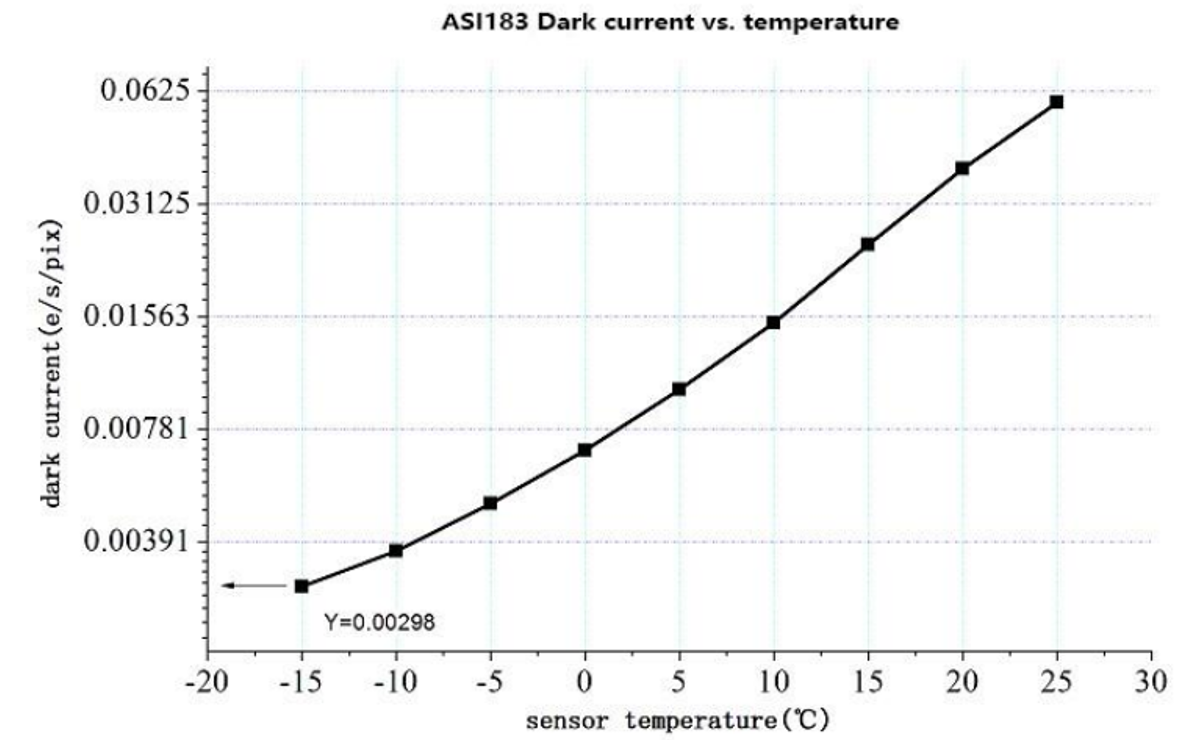
\includegraphics[scale=0.8]{4-experiment-design/img/mechanical/darkcurrent.png}
    	\caption{Dark current through the camera at various temperatures.}
	\label{fig:darkcurrent}
	\end{figure}

As an example, the SNR as affected by dark current at -10\,\textsuperscript{o}C versus 10\,\textsuperscript{o}C is\\

 SNR(-10\,\textsuperscript{o}C) =  $\frac{(\SI{6.16}{photons \per pixel \per sec})\times (0.84)\times (\SI{300}{s})}{\sqrt{(\SI{6.16}{photons \per pixel \per s})\times (0.84)\times (300s)+(\SI{0.00391}{e \per pixel \per s})\times (\SI{300}{s})+(\SI{1.6}{e})^2}}$ \\
 
 SNR(-10\,\textsuperscript{o}C) = 39.35\\
 
 SNR(10\,\textsuperscript{o}C) =  $\frac{(\SI{6.16}{photons \per pixel \per sec})\times (0.84)\times (300s)}{\sqrt{(\SI{6.16}{photons \per pixel \per s})\times (0.84)\times (\SI{300}{s})+(\SI{0.01563}{e \per pixel \per s})\times (\SI{300}{s})+(\SI{1.6}{e})^2}}$ \\

 SNR(10\,\textsuperscript{o}C) = 39.31\\


\paragraph{Optothermal stability}
Another important effect will be the how thermal stresses and subsequent deflections can affect the optics of the camera, in particular the index of refraction, and hence the quality of the collected data. Variation of solar flux over the time of flight and from the heat signatures of the BEXUS module will need to be considered. A thermoelastic analysis should be conducted in finite element analysis software to evaluate the effects of the thermal environment, and the implication of those results on the validity of the data should be investigated. \

\paragraph{Condensation}
Condensation may occur if air heated by the camera heating elements is able to condensate on the cold surfaces of the optics. This will deteriorate the quality of the detections and must also be mitigated.  \

\subsubsection{Thermal environment}
\paragraph{Atmosphere ambient conditions}
IRISC will ascend to and float in the stratosphere at an altitude of between 25 and 30\,km, after which it will experience altitude fluctuations of no more than 200\,m. This is the phase of flight during which the infrared camera will be operational and hence thermal control most necessary in ensuring sound optical performance. This part of the atmosphere is also characterised by relatively low temperatures. Based on the flights of number previous BEXUS missions seen in the graph of the atmosphere, it can be assumed that the atmospheric temperature during float will range between -70\,\textsuperscript{o}C and -50\,\textsuperscript{o}C. \\

	\begin{figure}[h!]
    \centering
    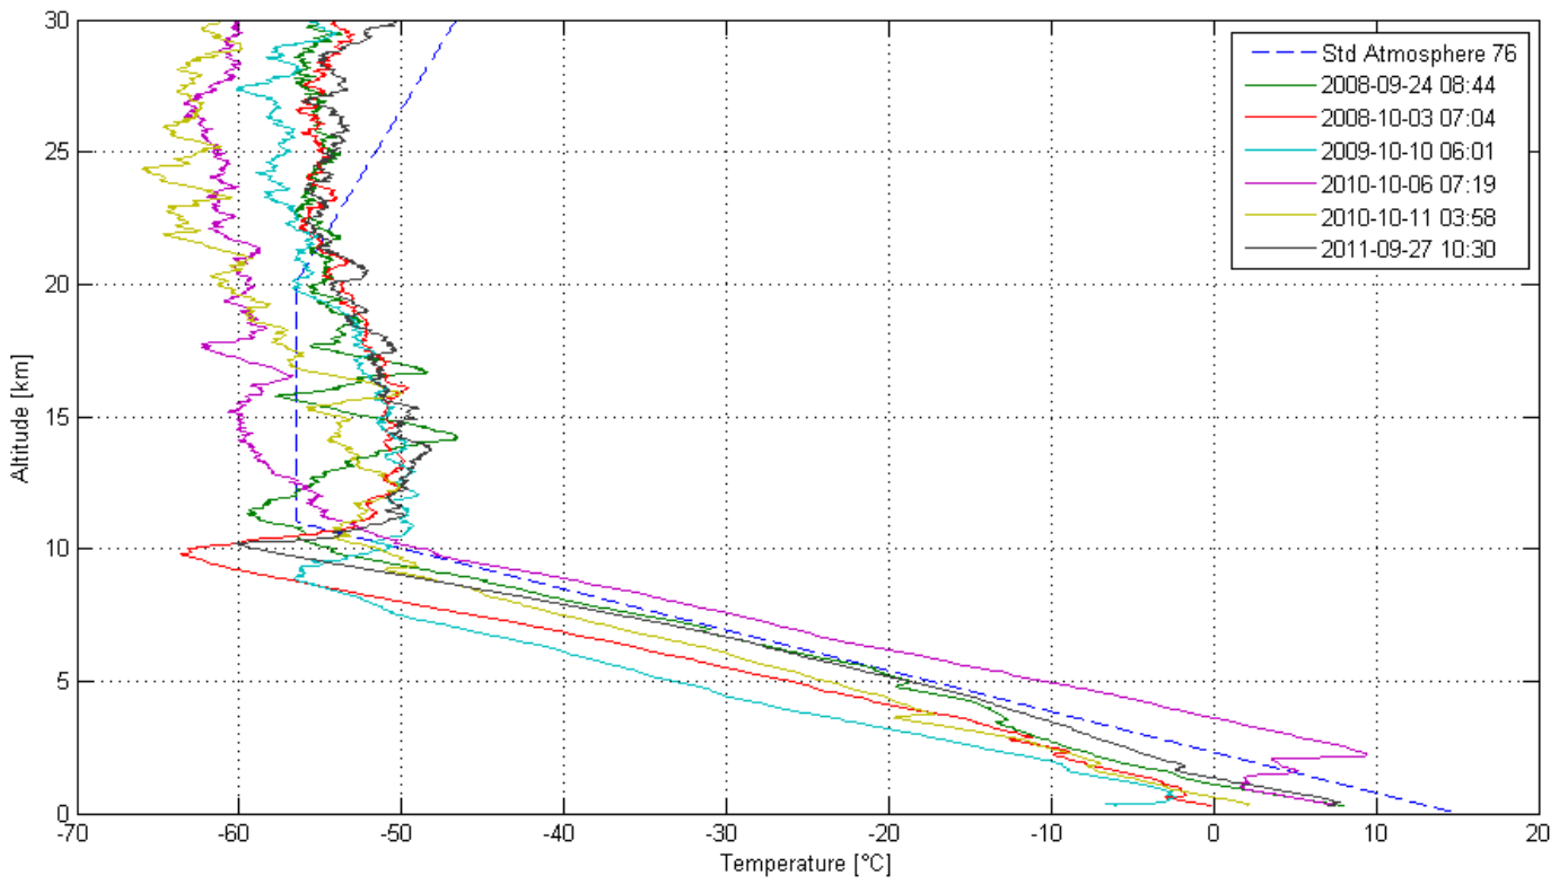
\includegraphics[scale=0.6]{4-experiment-design/img/mechanical/atmosphere.PNG}
	\caption{Temperature profile of the atmosphere.}
	\label{fig:atmosphere}
	\end{figure}
	
\begin{center}
  \begin{tabular}{ | l | c | r | }
    \hline
    \textbf{Flight phase} & \textbf{Expected temperature} & \textbf{Duration} \\ \hline
    Preparation  & 15 – 25\,\textsuperscript{o}C & 4 hours \\ \hline
    Launch pad wait & -15 – 0\,\textsuperscript{o}C & 3 hours \\ \hline
    Ascent phase  & -80 – 0\,\textsuperscript{o}C & 1.5 hours \\ \hline
    Float phase (25-30km) & -70 – -50\,\textsuperscript{o}C & 1 – 5 hours \\ \hline 
    Descent phase  & -80 – 0\,\textsuperscript{o}C & ~ 30 minutes \\ \hline
    Post-flight phase & -15 – 0\,\textsuperscript{o}C & 1 – 2 days \\ \hline
  \end{tabular}
\end{center}

\paragraph{Solar flux}

The extent of solar irradiance is characterised by several factors, including the sun’s height above the horizon, typically low for the polar latitudes that the balloon will be flying at, and the height in the atmosphere and atmospheric conditions, which will cause absorption and scattering of light. \\
The total solar irradiance, neglecting atmospheric effects, at the Esrange latitude of 68\textsuperscript{o} and assuming a launch date of the 15th of October is demonstrated in the following graph of direct solar radiation, with a peak of ~500\,kW/m\textsuperscript{2} at noon.\\

	\begin{figure}[h!]
    \centering
    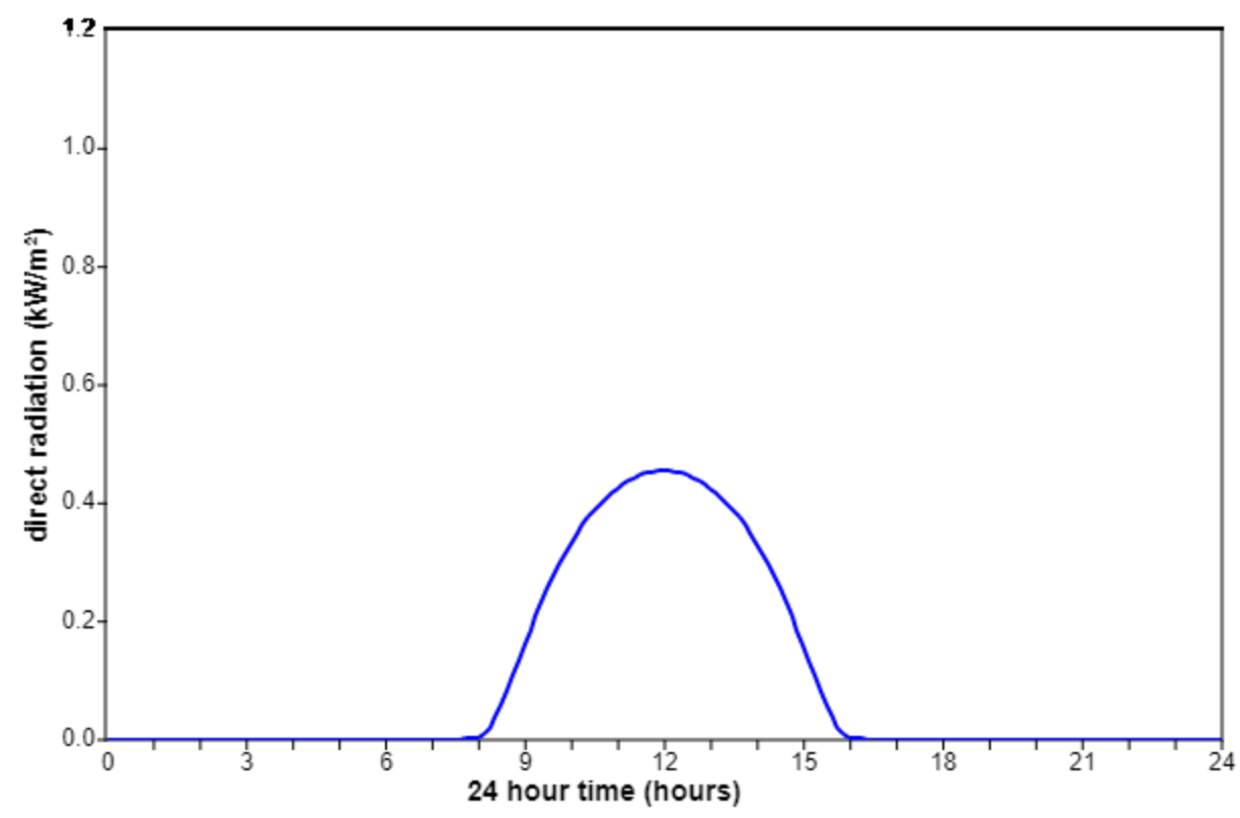
\includegraphics[scale=0.6]{4-experiment-design/img/mechanical/directradiation.png}
	\caption{Estimate of direct solar radiation at the top of the atmosphere.}
	\label{fig:directradiation}
	\end{figure}

The degree of attenuation of solar radiation through the atmosphere can be described using the Beer–Lambert law, which relates the transmittance of radiation to optical depth. For an atmosphere with properties that change exponentially with respect to altitude, the optical depth can be estimated to also change exponentially with respect to altitude. \


\subsubsection{Temperature requirements}

\begin{center}
  \begin{tabular}{ | l | c | }
    \hline
    \textbf{Component} & \textbf{Operating temperature} \\ \hline
    ASI183 camera  & -5 – 45\,\textsuperscript{o}C \\ \hline
    Camera module for Raspberry Pi 5MP 1080P & -20 – 80\,\textsuperscript{o}C \\ \hline
    Igarashi DC Gearmotor 33GN2738-132-GV-5 312:1  & 0* – 60\,\textsuperscript{o}C \\ \hline
    GYRO / ACCELEROMETER 3-AXIS  MPU-3050 & -20 – 105\,\textsuperscript{o}C \\ \hline 
    Electronics  & -5 – 60\,\textsuperscript{o}C \\ \hline
  \end{tabular}
\end{center}

*0\,\textsuperscript{o}C required to prevent condensation and subsequent freezing on the motors\\

As the ambient conditions are likely to be very cold, many of the components will need to be heated so that the electronics are able to operate. If the ambient conditions are assumed to be -70\,\textsuperscript{o}C, and the desired temperature for the components of 0\,\textsuperscript{o}C, heating will be needed to increase the temperature of components by up to  75\,\textsuperscript{o}C, a tolerance of 5\,\textsuperscript{o}C below the minimum operating temperature for the motors.\

\subsubsection{Thermal control}
In order to heat the electronics to the desired temperature, Polyimide Thermofoil Heaters supplied by Minco can be used, as they are lightweight, and commonly used to protect electronics from cold at high altitudes. A heater will be supplied for each of the three motors, for the camera, and for the electronics box. The heaters can be used to generate temperatures of up to 200\,\textsuperscript{o}C. Temperature sensors will be included next to the heaters to provide feedback that will allow the temperature to be controlled to the desired operating point. \\

The motor is 37.8\,mm long with a diameter of 33\,mm, so the 5572 heater with dimensions 12.7\,mm x 12.7\,mm and a resistance of 26.5\,\si{\ohm} is selected.\\

\begin{center}
 $P = \frac{\SI{5}{V}\textsuperscript{2}}{\SI{26.5}{\ohm}} = \SI{0.95}{W} $\\
\end{center}

The camera is 73.5\,mm long with a diameter of 78\,mm, so the 5587 heater with dimensions 31.8\,mm x 31.8\,mm and a resistance of 13.1\,\si{\ohm} is selected.\\

\begin{center}
 $P = \frac{\SI{5}{V}\textsuperscript{2}}{\SI{13.1}{\ohm}} = \SI{0.95}{W} $\\
\end{center}

The electronics box is 100\,mm x 100\,mm x 100\,mm, so the 5592 heater with dimensions 44.5\,mm x 44.5\,mm and a resistance of 26.3\,\si{\ohm} is selected.\\

\begin{center}
 $P = \frac{\SI{5}{V}\textsuperscript{2}}{\SI{26.3}{\ohm}} = \SI{0.95}{W} $\\
 \end{center}
 
\label{sec:4.6.5}

